\item

\begin{enumerate}
\item Durch identisches Umformen erhalten wir:

$$y'(y-2) = 3-x$$
$$\implies y' = \frac{3-x}{y-2}$$

\item Wir stellen für ein $c \in \mathbb{R}$ um:

$$y' = \frac{3-x}{y-2} = c$$
$$\implies y-2 = \frac{3-x}{c}$$
$$\implies y(x) = \frac{3-x}{c}+2$$
$$\implies y(x) = -\frac{1}{c}(x-3)+2$$

Es handelt sich bei den Isoklinen also um Geraden mit dem Anstieg $-\frac{1}{c}$, welche um $2$ Einheiten nach oben und um $3$ Einheiten nach rechts verschoben sind. Alle Isoklinen verlaufen durch den Punkt $(3,2)$.

\item Auf jedem Punkt einer solchen Gerade ist der Anstieg gleich. Der einzuzeichnende Anstieg des Richtungsfelds ist $c$, der zugehörige Anstieg der Isoklinen $m'=-\frac{1}{c}$. Es gilt daher $m'\cdot c = -1$, also steht der einzuzeichnende Anstieg orthogonal (senkrecht) zur Isoklinen.

\item Anders gesagt sind die Isoklinen daher Strahlen, welche radial vom Punkt $(3,2)$ ausgehen. Die Lösungskurven verlaufen senkrecht dazu, es handelt sich mithin um alle Kreise mit dem Ursprung $(3,2)$. Für den Anfangswert $y(4)=2$ beträgt der Radius des Kreises $r_{4,2} = \sqrt{(4-3)^2+(2-2)^2} = 1$, für $y(1)=1$ beträgt er $r_{4,2} = \sqrt{(1-3)^2+(1-2)^2} = \sqrt{5}$.

\item Das Online-Tool verwendet sogenannte numerische Lösungsverfahren, welche die wahre Lösungsfunktion aufgrund der Beschränktheit der Gleitkommazahlen nur approximativ (näherungsweise) ermitteln können. Ein einfaches solches Näherungsverfahren besteht darin, vom durch den Anfangswert gegebenen Punkt auszugehen (vgl. Abbildung \ref{fig4}). In finiten Schritten $\Delta x$ wird dann entsprechend dem momentanten Anstieg nach links bzw. nach rechts geschritten. Wo die Sprünge zu sehen sind, ist der Betrag des Anstiegs $|y'|$ sehr groß, sodass auch der Fehler bei einem Schritt $\Delta x$ größer wird. Am linken bzw. rechten Punkt des Kreises ist der Anstieg nicht mehr endlich, hier versagt das einfache Lösungsverfahren.

\end{enumerate}


\begin{figure}[ht]
	\centering
	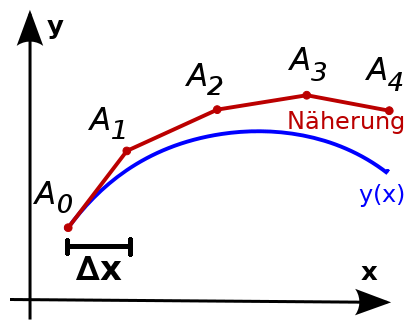
\includegraphics[width=0.4\textwidth]{../tex-snippets/ex-ode-slope-field-1-img-b.png}
	\caption{Einfaches numerisches Lösungsverfahren einer DGL der Ordnung 1 (Eulerverfahren). Es wird in endlich Schritten $\Delta x$ mit dem jeweiligen Anstieg von $A_0$ nach rechts zu $A_4$ geschritten. Die so erhaltene Kurve (rot) weicht von der tatsächlichen Lösungskurve (blau) ab. Je größer der Anstieg der Lösungskurve, desto größer ist der Fehler bei gegebenen $\Delta x$.}
	\label{ex-ode-slope-field-1-img-b}
\end{figure}

